% context: 9th-grade physics classwork, Unit 2 kinematics, Giancoli 2-2 and 2-3
% topic: average speed vs average velocity, instantaneous velocity as the limit of
%        shorter and shorter intervals, average velocity of each leg of a path drawn
%        as vectors on a grid; follows 2-1HW (the hallway walk returns with times)
% structure: two pages; page 1 average speed and velocity in one dimension,
%        page 2 instantaneous velocity from a data table, then vectors on a grid.
%        No 2-D vector addition yet.
\documentclass[12pt, twoside]{article}
%\documentclass[12pt, twoside]{article}
\usepackage[letterpaper, margin=1in, headsep=0.2in]{geometry}
\setlength{\headheight}{0.6in}
%\usepackage[english]{babel}
\usepackage[utf8]{inputenc}
\usepackage{microtype}
\usepackage{amsmath}
\usepackage{amssymb}
%\usepackage{amsfonts}
\usepackage[nomessages]{fp} %\FPeval{\var-name}{2*sin(pi/6)}
\usepackage{siunitx} %units in math. eg 20\milli\meter
\usepackage{yhmath} % for arcs, overparenth command
\usepackage{tikz} %graphics
\usetikzlibrary{quotes, angles, arrows, arrows.meta}
\usepackage{graphicx} %consider setting \graphicspath{{images/}}
\usepackage{parskip} %no paragraph indent
\usepackage{enumitem}
\usepackage{multicol}
\usepackage{venndiagram}

\usepackage{fancyhdr}
\pagestyle{fancy}
\fancyhf{}
\renewcommand{\headrulewidth}{0pt} % disable the underline of the header
\raggedbottom
\hfuzz=2mm %suppresses overfull box warnings

\usepackage{hyperref}
\usepackage{float}

\title{Physics}
\author{Chris Huson}
\date{October 2026}

\fancyhead[LE]{\thepage}
\fancyhead[RO]{\thepage \\ Nickname: \hspace{2.25cm} \,\\ \,}
\fancyhead[LO]{La Scuola d'Italia / Huson / Physics \\* 16 October 2026}

\begin{document}

\subsubsection*{2.2 Classwork: Average and Instantaneous Velocity}

\textbf{Reference (provided).} \quad
average speed $= \dfrac{\text{distance}}{\text{time}}$ \quad
average velocity $\bar{v} = \dfrac{\text{displacement}}{\text{time}}$
\quad 1 h = 3600 s

\vspace{0.2cm}

\begin{enumerate}[itemsep=0.5cm]

\item Swimming world records are set in a 50 m pool. The race distances are exact,
  so give four significant figures.
  \begin{enumerate}[itemsep=1.1cm]
    \item The 50 m freestyle record is 20.91 s, one length of the pool. Find the
      swimmer's average speed and average velocity.
    \item The 100 m freestyle record is 46.40 s, two lengths: down the pool and back
      to the starting wall. Find the swimmer's average speed and average velocity.
  \end{enumerate}
  \vspace{1.0cm}

\item The hallway walk from 2.1, now with a stopwatch. Take east as positive.

  \begin{center}
  \renewcommand{\arraystretch}{1.35}
  \begin{tabular}{| c | c | c | p{4.2cm} |}
    \hline
    Leg & Displacement & Time & Average velocity \\ \hline
    1 & 8.0 m east & 4.0 s & \\ \hline
    2 & 5.0 m west & 5.0 s & \\ \hline
    3 & 7.0 m west & 5.0 s & \\ \hline
  \end{tabular}
  \end{center}

  \begin{enumerate}[itemsep=1.1cm]
    \item Fill in the average velocity of each leg. Give each one a sign.
    \item For the whole walk, find the average speed and the average velocity. Why
      is one so much smaller than the other?
  \end{enumerate}
  \vspace{1.1cm}

\item The fastest Frecciarossa trains run from Roma Termini to Milano Centrale,
  about 570 km by rail, in 2 h 59 min without stopping.
  \begin{enumerate}[itemsep=1.5cm]
    \item Find the train's average speed in km/h.
    \item On the way, the display in the carriage reads 300 km/h. Is that an average
      or an instantaneous speed? Give one reason the average is lower.
  \end{enumerate}

\newpage

\item \textbf{Instantaneous velocity.} A cart is released from rest at the top of a
  tilted Vernier track. Graphical Analysis gives its position at these times.

  \begin{center}
  \renewcommand{\arraystretch}{1.3}
  \begin{tabular}{| c | c | c | c | c | c |}
    \hline
    $t$ (s) & 1.00 & 1.05 & 1.10 & 1.50 & 2.00 \\ \hline
    $x$ (m) & 0.250 & 0.276 & 0.303 & 0.563 & 1.000 \\ \hline
  \end{tabular}
  \end{center}

  \begin{enumerate}[itemsep=0.4cm]
    \item Find the average velocity over each time interval.

      \vspace{0.1cm}
      \renewcommand{\arraystretch}{1.4}
      \begin{tabular}{| c | c | c | p{3.6cm} |}
        \hline
        Interval & $\Delta t$ (s) & $\Delta x$ (m) & $\bar{v}$ (m/s) \\ \hline
        1.00 s to 2.00 s & & & \\ \hline
        1.00 s to 1.50 s & & & \\ \hline
        1.00 s to 1.10 s & & & \\ \hline
        1.00 s to 1.05 s & & & \\ \hline
      \end{tabular}
    \item As the interval gets shorter, what value is $\bar{v}$ getting close to?
      That is the cart's instantaneous velocity at $t = 1.00$ s. \vspace{0.5cm}
    \item Why can we not keep shrinking the interval to get a better answer from
      this data? \vspace{0.3cm}
  \end{enumerate}

\item A soccer player runs a drill: 6.0 m east in 2.0 s, then 4.0 m north in 2.0 s,
  then 6.0 m west in 3.0 s. East is $+x$ and north is $+y$.

  \begin{minipage}[t]{0.56\linewidth}
    \vspace{0pt}
    \begin{enumerate}[itemsep=1.3cm]
      \item On the path grid, draw the drill as three displacement vectors, each
        starting where the last one ended. Number them 1, 2, 3.
      \item Find the average velocity of each leg, with its direction. Draw each one
        as an arrow from the origin of the velocity grid.
      \item For the whole drill, find the average speed and the average velocity.
        The path grid shows where the player finishes.
    \end{enumerate}
  \end{minipage}
  \hfill
  \begin{minipage}[t]{0.4\linewidth}
    \vspace{0pt}
    \centering
    \begin{tikzpicture}[scale=0.45]
      \draw[gray!40, thin, step=1] (-1,-1) grid (8,5);
      \draw[->, thick] (-1.3,0) -- (8.6,0) node[right]{\small $x$};
      \draw[->, thick] (0,-1.3) -- (0,5.6) node[above]{\small $y$};
      \foreach \x in {2,4,6,8} \node[below] at (\x,0) {\scriptsize \x};
      \foreach \y in {2,4} \node[left] at (0,\y) {\scriptsize \y};
      \node[below] at (3.5,-1.3) {\small path: 1 square = 1 m};
      % Solution path — uncomment to see the answer
      %\draw[->, very thick] (0,0) -- (6,0) node[midway, above]{\small 1};
      %\draw[->, very thick] (6,0) -- (6,4) node[midway, right]{\small 2};
      %\draw[->, very thick] (6,4) -- (0,4) node[midway, above]{\small 3};
    \end{tikzpicture}

    \vspace{0.15cm}
    \begin{tikzpicture}[scale=0.45]
      \draw[gray!40, thin, step=1] (-4,-1) grid (4,3);
      \draw[->, thick] (-4.3,0) -- (4.6,0) node[right]{\small $x$};
      \draw[->, thick] (0,-1.3) -- (0,3.6) node[above]{\small $y$};
      \foreach \x in {-4,-2,2,4} \node[below] at (\x,0) {\scriptsize \x};
      \foreach \y in {2} \node[left] at (0,\y) {\scriptsize \y};
      \node[below] at (0,-1.3) {\small velocity: 1 square = 1 m/s};
      % Solution velocity vectors — uncomment to see the answer
      %\draw[->, very thick] (0,0) -- (3,0) node[midway, above]{\small 1};
      %\draw[->, very thick] (0,0) -- (0,2) node[midway, right]{\small 2};
      %\draw[->, very thick] (0,0) -- (-2,0) node[midway, above]{\small 3};
    \end{tikzpicture}
  \end{minipage}

\end{enumerate}
\end{document}
